\documentclass{article}
\usepackage[utf8]{inputenc}
\usepackage[T1]{fontenc}
\usepackage[export]{adjustbox}
\usepackage{mathtools,amsthm,amssymb,icomma,upgreek,xfrac,enumerate, bbm,titlesec,lmodern,polski,derivative,multicol,titling,graphicx,url,amsmath,caption,lipsum,float,longtable,booktabs}
\usepackage[table,xcdraw]{xcolor}
\usepackage[hidelinks,breaklinks,pdfusetitle,pdfdisplaydoctitle]{hyperref}
\setlength{\droptitle}{-1cm}
\mathtoolsset{showonlyrefs,mathic}
\title{Analiza sygnałów raport 2}
\author{Joanna Kołaczek}
\date{21.06.2022}
\newtheoremstyle{break}
{\topsep}{\topsep}%
{\normalfont}{}%
{\bfseries}{}%
{\newline}{}%
\theoremstyle{break}
\newtheorem{zadanie}{Zadanie} 
\newtheorem*{rozwiazanie}{Rozwiązanie}

\titleformat*{\section}{\LARGE\bfseries}
\titleformat*{\subsection}{\Large\bfseries}
\titleformat*{\subsubsection}{\large\bfseries}
\titleformat*{\paragraph}{\large\bfseries}
\titleformat*{\subparagraph}{\large\bfseries}

%% KOMENDY:
\newcommand*{\e}{\mathrm{e}}
\newcommand{\hyline}[2]{%
	$#1$\> --\kern.5em #2 \\}


%% OPERATORY:
% `\diff` od „differential”, czyli odpowiednika słowa „różniczka” w języku
% angielskim.
\DeclareMathOperator{\diff}{d\!}
\newcommand{\indep}{\perp \!\!\! \perp}
\DeclareMathOperator{\EX}{\mathbb{E}}
\newcommand*{\E}{\mathrm{e}}


%nowe
\usepackage[letterpaper,margin=1in]{geometry}
\usepackage{array}

\newcommand\myarray[1]{%
	\begingroup
	\renewcommand\arraystretch{1.33}
	\left\{ \begin{array}{@{}l@{}} #1 \end{array} \right.
	\endgroup}


\begin{document}

\section*{Zadanie 2}
\textbf{Procesem Wienera} (ruchem Browna) nazywamy proces stochastyczny $B = (B_t)_{t\geq0}$, taki że:
\begin{itemize}
	\item $B_0=0$.
	\item $B$ ma niezależne przyrosty.
	\item $B_t-B_s\sim N(0,~t-s)$, dla $0\leq s<t$.
	\item $B$ ma trajektorie ciągłe z prawdopodobieństwem 1.
\end{itemize}
W zadaniu będziemy posługiwać się jego zmodyfikowaną wersją:
$$B_t^x=B_t^0+x,$$
Gdzie $B_t^0$ to klasyczny ruch Browna. Oznacza to tyle, że proces $B_t^x$ rozpoczyna się w punkcie $x$. Chcąc uzyskać jego numeryczne przybliżenie przy pomocy symulacji komputerowej, wykorzystamy następujący algorytm:
\\ \\
Algorytm(0)
\begin{enumerate}
	\item $B_0^x=x$
	\item $B_{i+1}^x=B_{i}^x+dt^{\frac{1}{2}}\psi_i$
\end{enumerate}
gdzie $\psi_i\sim N(0,1),\quad i.i.d$, natomiast $dt$ to najmniejszy krok czasowy.\\ \\ 
Będziemy badać średni czas wyjścia z  przedziału $[a,b]$, dla $x\in[a,b]$. Oznaczmy go jako $$\mathbb{E}\tau_x \mathrm{,~gdzie~}\tau_x:=\inf\{t\geq0:B_t^x\notin(a,b)\}.$$ 
Ponieważ na komputerze nie jest możliwe wykonanie symulacji procesu Wienera w czasie ciągłym, ustalamy najmniejszy krok czasowy $dt$, potrzebny do zastosowania metody numerycznej. Aby móc jak najlepiej oszacować średni czas wyjścia, powtarzamy $n$ razy symulację dla danego~$x$.\\ \\
Algorytm(1):
\begin{enumerate}
	\item Ustal punkt startowy $x$, najmniejszy krok czasowy $dt$, liczbę powtórzeń symulacji $n$ oraz granice przedziału $a$ i $b$.
	\item Jeżeli $x=a$ lub $x=b$ zwróć 0.
	\item Ustal $T=0$ 
	\item Generuj trajektorię procesu Wienera $B_t^x$ dopóki $B_t^x\leq a$ lub $B_t^x\geq b$.
	\item Zwiększ $T$ o ilość kroków czsowych $dt$, które mineły do tego momentu.
	\item Powtórz kroki 4-5 $n$ razy.
	\item Zwróć $\frac{T}{n}$.
\end{enumerate}
Chcąc zbadać zależność średniego czasu wyjścia od odległości punktu startowego $x$ do granic przedziału $[a,b]$ musimy ustalić $dx$, czyli różnicę między kolejnymi początkowymi $x \in [a,b]$.\\ \\ 
Algorytm(2):
\begin{enumerate}
	\item Ustal różnicę $dx$, najmniejszy krok czasowy $dt$, liczbę powtórzeń symulacji $n$, oraz granice przedziału $a$ i $b$.
	\item Stwórz pusty wektor $y$.
	\item Stwórz wektor $v$, początkowych $x$-ów należących do przedziału $[a,b]$, tak aby $v[i+1]-v[i]=dx$.
	\item Dla każdego elementu z wektora $v$ oblicz średni czas wyjścia (Algorytm(1)) i wstaw otrzymany wynik do wektora~$y$.
	\item Zwróć $y$
\end{enumerate}
Mając powyższe informacje, możemy przeprowadzić symulację. Rozważmy przypadki dla $n=10^3$ i $n=10^5$, $dt=0.1$, $dx=1$, $a=50$, $b=150$. Otrzymujemy wyniki widoczne na rys. \ref{fig:1} i rys. \ref{fig:2}
\begin{figure}[H]
	\begin{multicols}{2}
	\begin{center}
	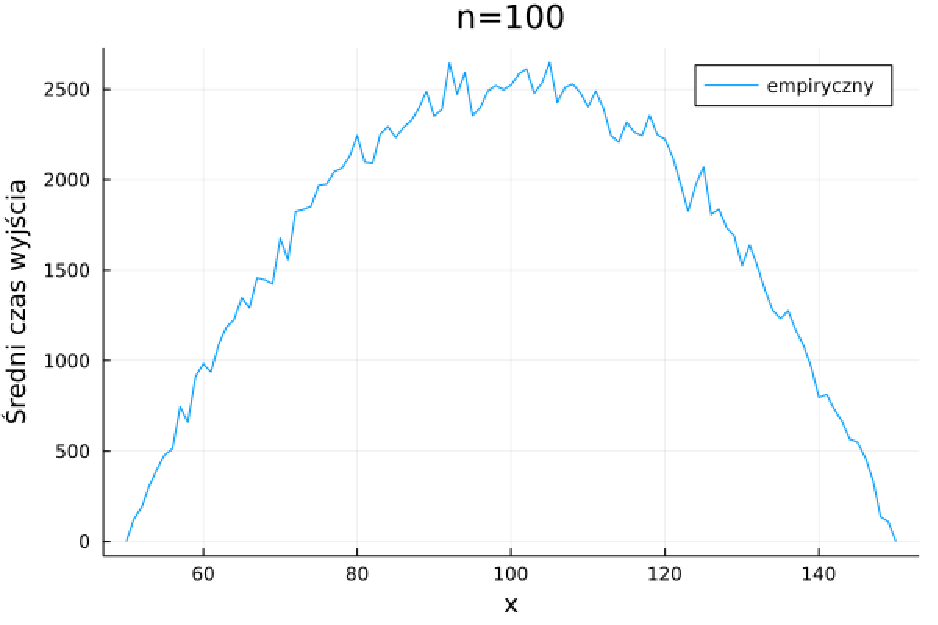
\includegraphics[scale=0.30]{time100.pdf}
	\caption{}
	\label{fig:1}
	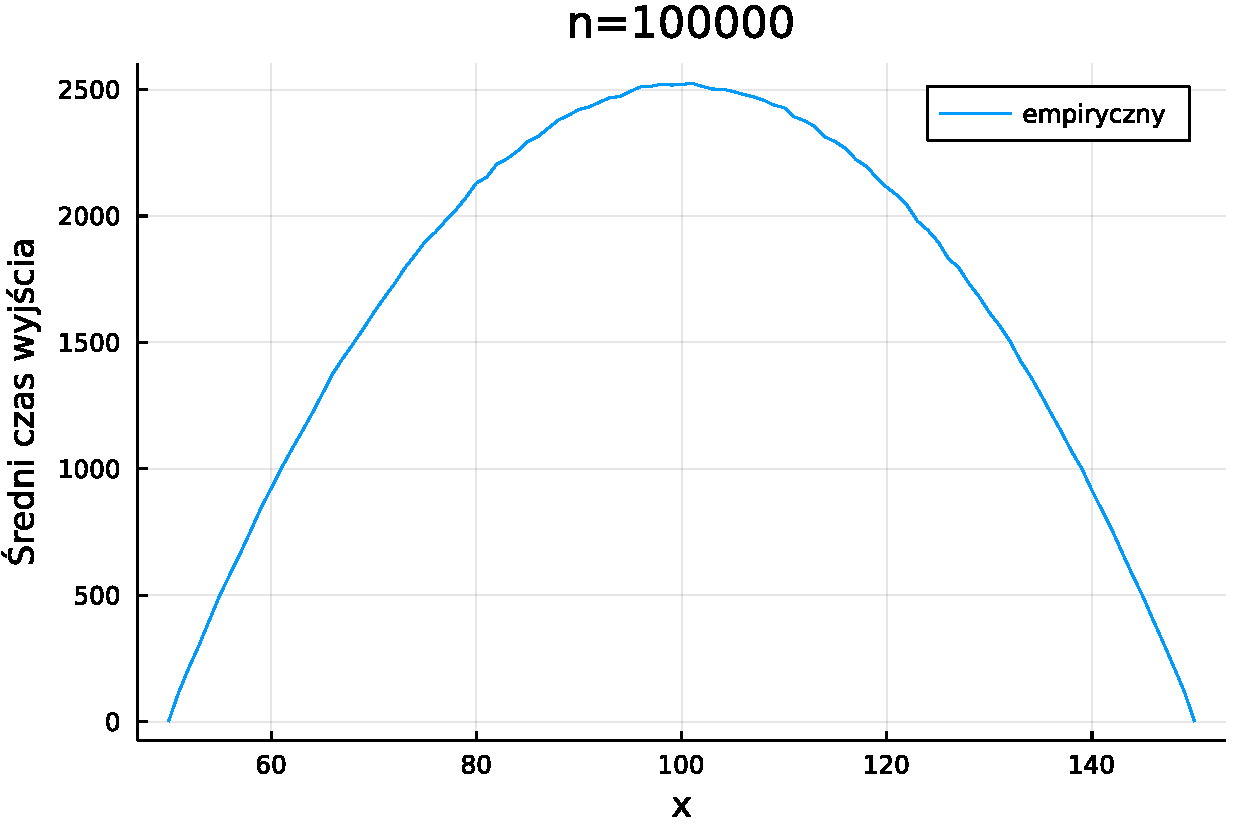
\includegraphics[scale=0.30]{time100000.pdf}
	\caption{}
	\label{fig:2}
	\end{center}
	\end{multicols}
\end{figure}
Spróbujemy aproksymować funkcję, która opisuje otrzymane wyniki. Po kształcie wykresu przypuszczamy, że może to być wielomian co najmniej stopnia II na przedziale $[a,b]$. Wiemy również, że jego zera znajdują się w punktach $a$ oraz $b$, ponieważ czas wyjścia w przypadku gdy $x=a$ lub $x=b$, będzie wynosił 0. Załóżmy więc, że jest to funkcja kwadratowa, po zapisaniu w postaci kwadratowej wygląda następująco:
$$f(x)=\alpha(x-a)(x-b),$$
gdzie $\alpha$ jest szukanym współczynnikiem. W rozważanym przez nas przypadku:
$$f(x)=\alpha(x-50)(x-150).$$
Aby znaleźć współczynnik $\alpha$ użyjemy modułu \textit{numpy.polyfit}. Dla przypadku z $n=10^3$ otrzymujemy $\alpha~=~1.012$, natomiast dla $n=10^5$, $\alpha=-1.001$. Na wykresie \ref{fig:a} widzimy jak współczynnik $\alpha$ zmienia się wraz ze wzrostem $n$. Możemy przypuścić, że $\lim\limits_{n\rightarrow\infty}c=-1$. Podobnie średnia ze stu powtórzeń algorytmu(2) dla $n=1000$ wraz z aproksymacją \textit{numpy.polyfit} wskazała, że $\alpha=1$. Ostatecznie otrzymujemy:
$$f(x)=-(x-50)(x-150).$$
\begin{figure}[H]
	\begin{center}
		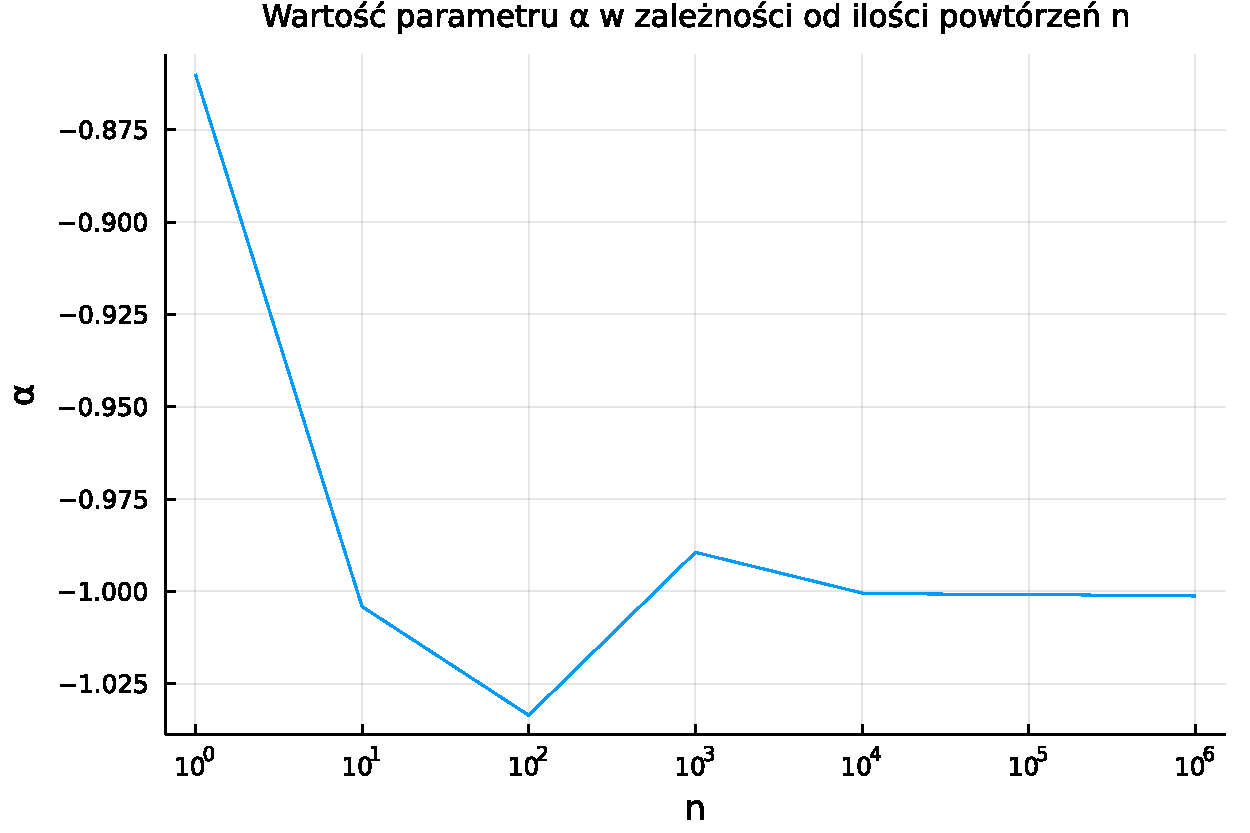
\includegraphics[scale=0.30]{alpha.pdf}
		\caption{}
		\label{fig:a}
	\end{center}
\end{figure}
Zestawienie funkcji empirycznej z teoretyczną znajduje się na rys. \ref{fig:3} oraz rys. \ref{fig:4}.
\begin{figure}[H]
	\begin{multicols}{2}
		\begin{center}
			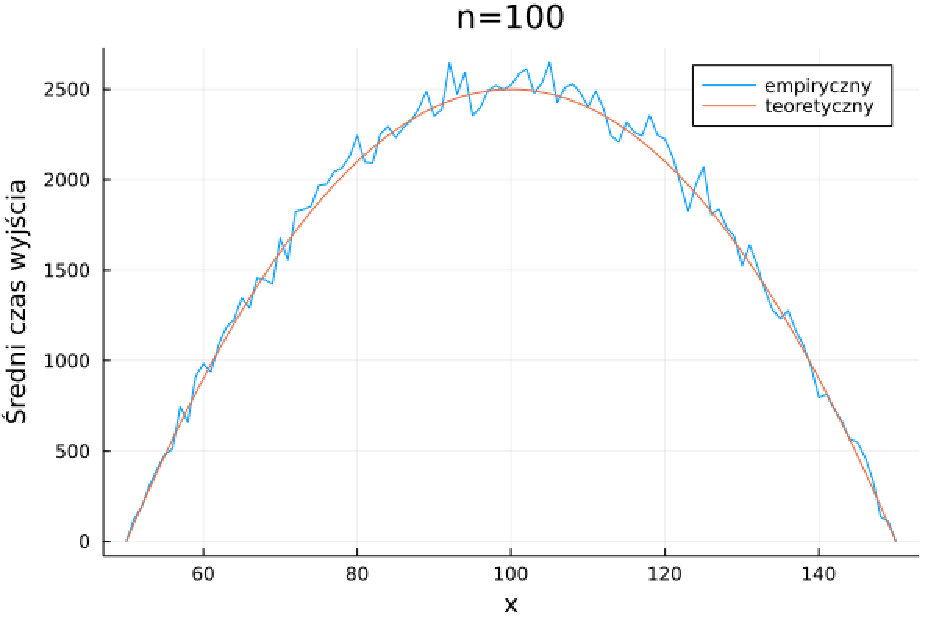
\includegraphics[scale=0.30]{time100poly.pdf}
			\caption{}
			\label{fig:3}
			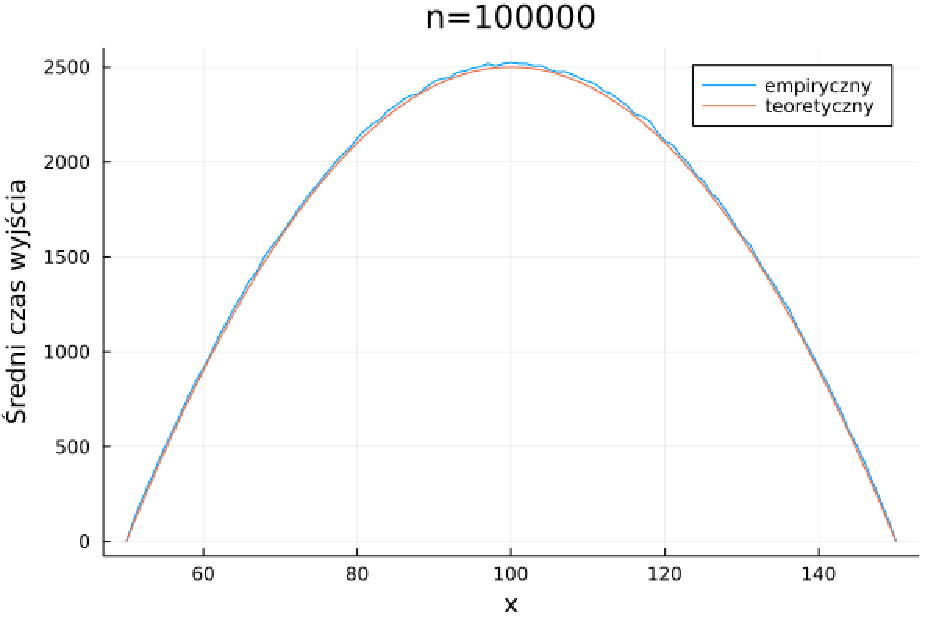
\includegraphics[scale=0.30]{time100000poly.pdf}
			\caption{}
			\label{fig:4}
		\end{center}
	\end{multicols}
\end{figure}
Przejdziemy teraz do szacowania, że wyjście nastąpiło przez granicę $b$, czyli:
$$P(B_{\tau^x}^x=b).$$
Jako, że symulacja działa w czasie dyskretnym, do określenia prawdopodobieństwa użyjemy wzoru:
$$P(B_{\tau^x}^x\geq b).$$
Postępujemy podobnie jak w przypadku szukania średniego czasu wyjścia.\\ \\
Algorytm(3):
\begin{enumerate}
	\item Ustal punkt startowy $x$, najmniejszy krok czasowy $dt$, liczbę powtórzeń symulacji $n$  oraz granice przedziału $a$ i $b$.
	\item Jeżeli $x=a$ zwróć 0.
	\item Jeżeli $x=b$ zwróć 1.
	\item Ustal $k=0$ 
	\item Generuj trajektorię procesu Wienera $B_t^x$ dopóki $B_t^x\leq a$ lub $B_t^x\geq b$.
	\item Jeśli $w\geq b$ zwiększ $k$ o jeden.
	\item Powtórz kroki 5-6 $n$ razy.
	\item Zwróć $\frac{k}{n}$.
\end{enumerate}
Analogicznie tworzymy algorytm, mający na celu zbadanie zależności między prawdopodobieństwem wyjścia przez $b$ a początkowym $x\in [a,b]$.\\ \\ 
Algorytm(4):
\begin{enumerate}
	\item Ustal różnicę $dx$, najmniejszy krok czasowy $dt$, liczbę powtórzeń symulacji $n$, oraz granice przedziału $a$ i $b$.
	\item Stwórz pusty wektor $y$.
	\item Stwórz wektor $v$, początkowych $x$-ów należących do przedziału $[a,b]$, tak aby $v[i+1]-v[i]=dx$.
	\item Dla każdego elementu z wektora $v$ oblicz prawdopodobieństwo wyjścia przez $b$ (Algorytm(3)) i wstaw otrzymany wynik do wektora~$y$.
	\item Zwróć $y$
\end{enumerate}
Korzystając z algorytmu 3 i 4, przeprowadzimy symulację dla $n=10^3$ i $n=10^5$, $dt=0.1$, $dx=1$, $a=50$, $b=150$. Otrzymujemy wyniki widoczne na rys. \ref{fig:5} i rys. \ref{fig:6}
\begin{figure}[H]
	\begin{multicols}{2}
		\begin{center}
			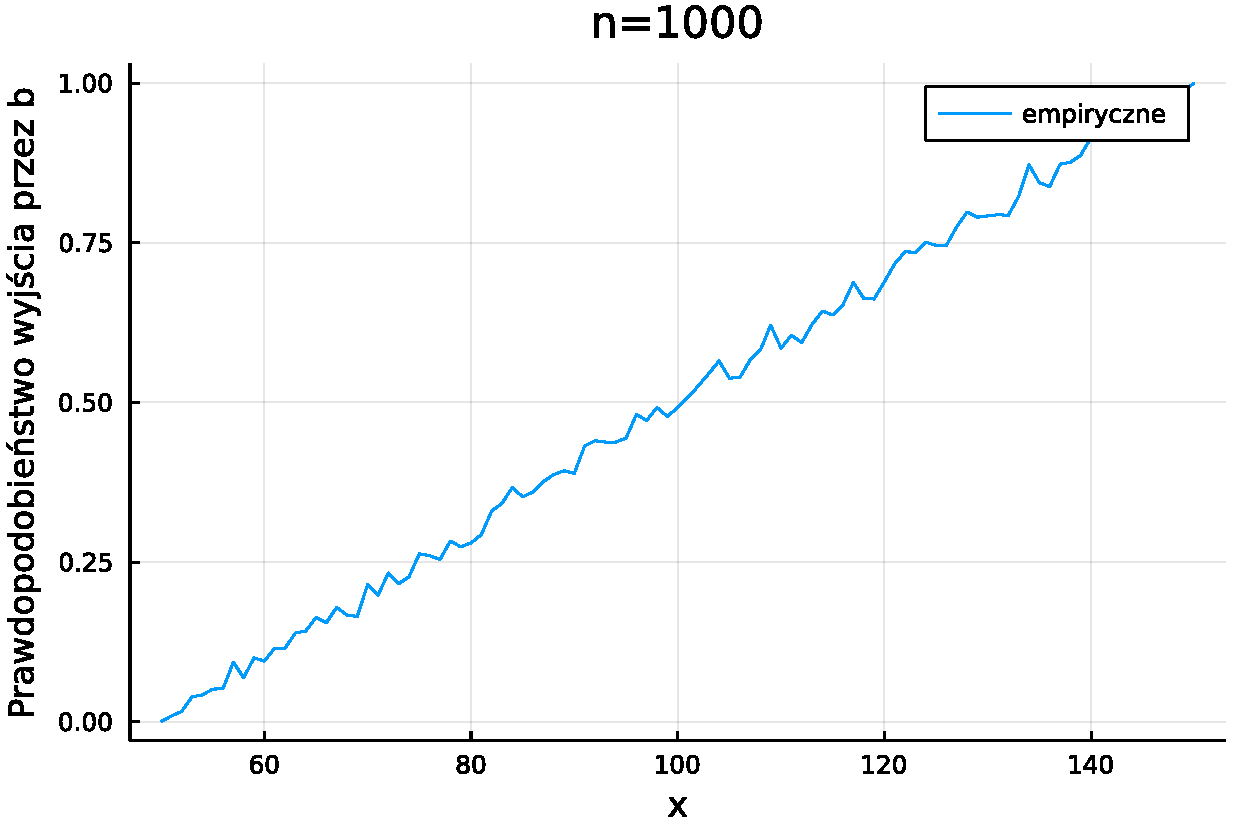
\includegraphics[scale=0.30]{prob100.pdf}
			\caption{}
			\label{fig:5}
			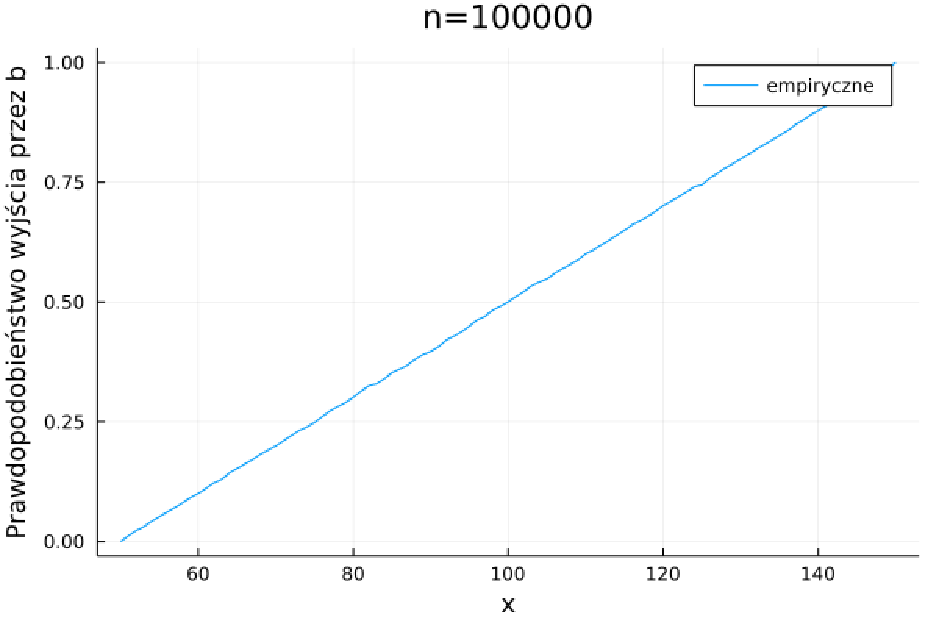
\includegraphics[scale=0.30]{prob100000.pdf}
			\caption{}
			\label{fig:6}
		\end{center}
	\end{multicols}
\end{figure}
Po kształcie wykresu spodziewamy się, że jest to funkcja liniowa. Kiedy początkowe $x=a$, prawdopodobieństwo wyjścia przez $b$ wynosi 0, natomiast gdy początkowe $x=b$, prawdopodobieństwo to będzie wynosić~1. Znając dwa punkty przez które przechodzi funkcja liniowa $f(x)=\beta x+\gamma$, gdzie $\beta$ i $\gamma$ są szukanymi parametrami, możemy wyprowadzić ogólny wzór rozwiązując następujący układ równań:
\[
\myarray{\beta a + \gamma = 0\\ \beta b + \gamma = 1}
\Leftrightarrow
\myarray{\beta = \frac{-1}{a-b} \\ \gamma = \frac{a}{a-b}}
\]
Zatem:
$$f(x)=-\frac{1}{a-b}x + \frac{a}{a-b}$$
Podstawiając nasze dane ($a=50$, $b=150$), otrzymujemy:
$$f(x)=\frac{1}{100}x-\frac{1}{2}$$
Sprawdzamy, czy moduł \textit{numpy.polyfit} da nam pdobny rezultat, przy jego pomocy otrzymujemy:
$$f(x)=0.00997x-0.497 \quad \mathrm{dla} \quad n=10^3$$
$$f(x)=0.01x-0.5 \quad \mathrm{dla} \quad n=10^5$$
Co zgadza się z naszymi teoretycznymi obliczeniami (im większe $n$ tym większa dokładność). Na wykresach zestawienie empirycznej i teoretycznej funkcji prezentuje się następująco (rys. \ref{fig:7} i rys. \ref{fig:8}):
\begin{figure}[H]
	\begin{multicols}{2}
		\begin{center}
			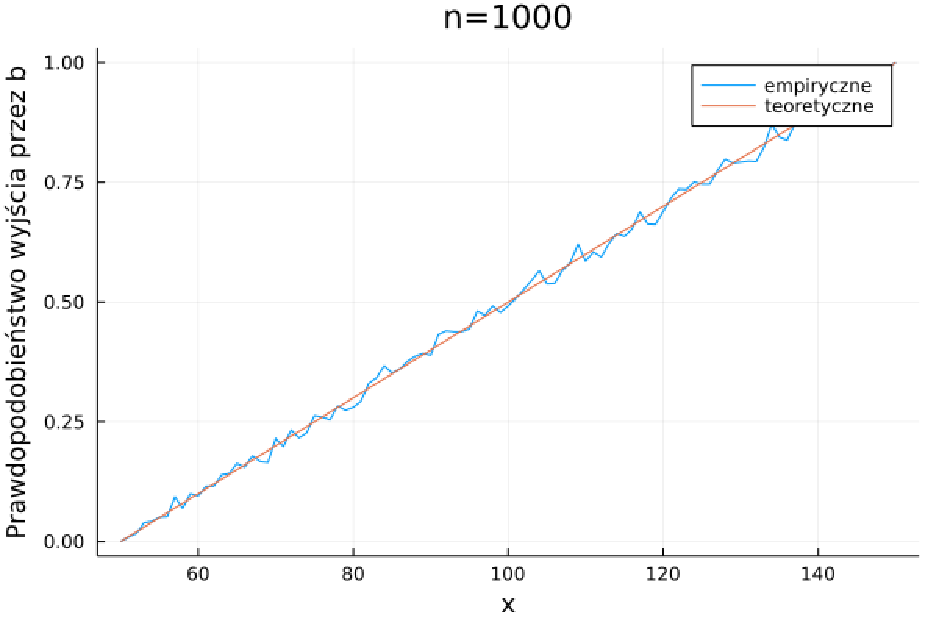
\includegraphics[scale=0.30]{prob100poly.pdf}
			\caption{}
			\label{fig:7}
			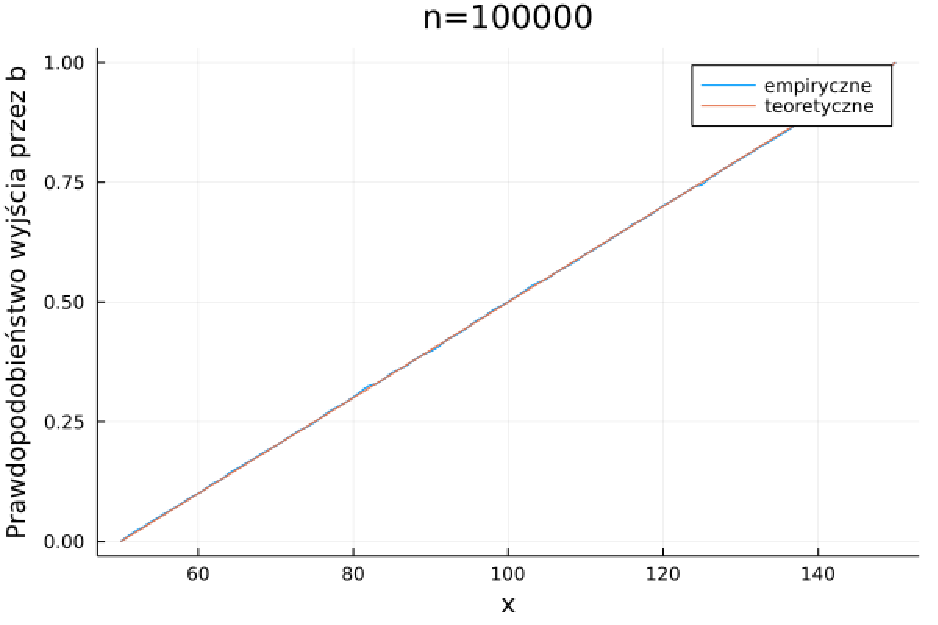
\includegraphics[scale=0.30]{prob100000poly.pdf}
			\caption{}
			\label{fig:8}
		\end{center}
	\end{multicols}
\end{figure}

\subsection*{Podsumowanie}
W zadaniu szukaliśmy zależności, między średnim czasem wyjścia z przedziału $[a,b]$ oraz prawdopodobieństwem, że wyjście to nastąpi przez $b$, a wartością początkową $x$. Musimy jednak pamiętać, że przeprowadzając symulację metodą numeryczną, dostaniemy jedynie przybliżone zachowanie procesu Wienera. Aby uzyskać rzeczywisty efekt, nasz minimalny krok czasowy $dt$ musiałby dążyć do zera. Żeby wyniki były jak najbardziej rzetelne, musi zostać spełniony następujący warunek:
 $$dt<<|a-b|.$$ 
Należy jednak pamiętać, że dla ustalonego $dt$, zwiększając różnicę $|a-b|$, zwiększa się również czas wykonywania symulacji, dlatego mając ograniczone warunki, nie powinna być ona zbyt duża. Wykonując więcej powtórzeń ($n$), również poprawiamy dokładność otrzymanych wyników, jednak tutaj podobnie dobrze jest zachować umiar.
\\ \\
Obserwując średni czas wyjścia, w zależności od początkowego $x$, widzimy że rośnie on wraz z odległością do bliższej granicy $a$ lub $b$. Będzie on najdłuższy, kiedy $|x-a|=|x-b|$, czyli dla $x=\frac{a+b}{2}$. Wtedy też prawdopodobieństwo wyjścia przez granicę $b$:
 $$\beta=P(B_{\tau^x}^x=b),$$
jest równe prawdopodobieństwu wyjścia przez granicę $a$: $$\alpha=1-\beta=P(B_{\tau^x}^x=a),$$
$$\alpha=\beta=\frac{1}{2}.$$

\end{document}